\begin{frame}
  \frametitle{Motivation \& Contribution}
  \vspace{2ex}
  \ribbon[\paperwidth][black][VectorPink]{ \centering \textbf{We develop KFAC for, and apply it to, loss functions with differential operators.} }
  \begin{columns}
    \begin{column}[b]{0.37\linewidth}
      \begin{itemize}
        \uncover<2->{
        \item Goal: Learn PDE solution
          \begin{align*}
            \hat{\gL} u(\vx)
            &=
              f(\vx) \qquad \vx \in \Omega
            \\
            u(\vx)
            &=
              g(\vx) \qquad \vx \in \partial \Omega
          \end{align*}
          % \item E.g.\,Poisson equation
          %   \begin{align*}
    %     \hat{\gL} = -\Delta_{\vx} = -\Tr(\nabla_{\vx}^2)
    %   \end{align*}

        \item Ansatz: Neural net $u_{\vtheta}(\vx)$
        }
        \uncover<3->{
        \item Sample $\vx_n \sim \Omega$, $\vx_n^{\text{b}} \sim \partial \Omega$
        }
      \end{itemize}
    \end{column}
    \begin{column}[b]{0.53\linewidth}
      \vspace{1ex}
      \centering \only<1-3>{%
        \begin{animateinline}[loop, autoplay]{1.0}
          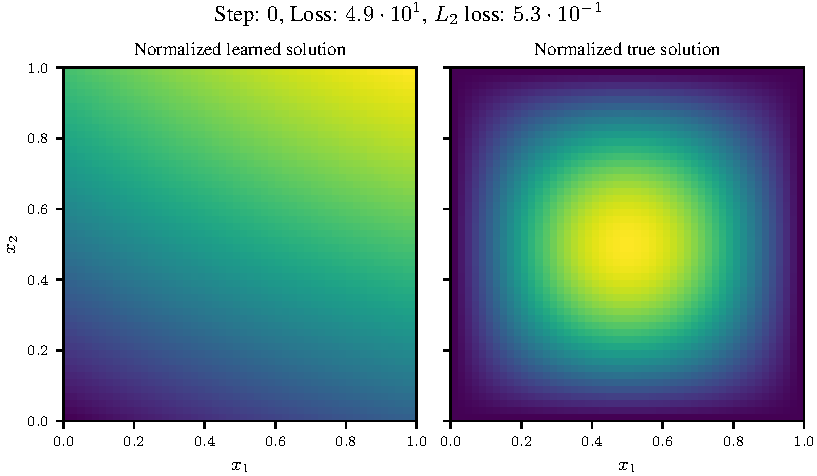
\includegraphics[width=\linewidth]{../kfac_pinns_exp/exp42_visualize_solutions/visualize_solution/SGD/poisson_2d_sin_product_mlp-tanh-64_SGD_step0000000.pdf}%
          \newframe[1.0]%
          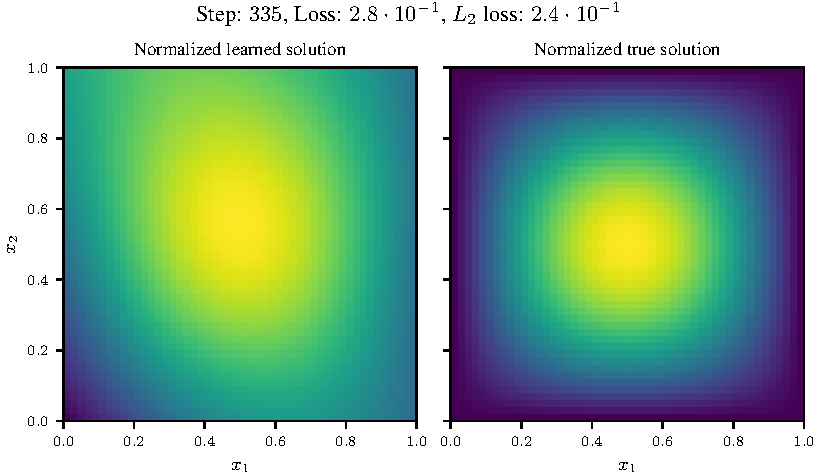
\includegraphics[width=\linewidth]{../kfac_pinns_exp/exp42_visualize_solutions/visualize_solution/SGD/poisson_2d_sin_product_mlp-tanh-64_SGD_step0000335.pdf}%
          \newframe[1.0]%
          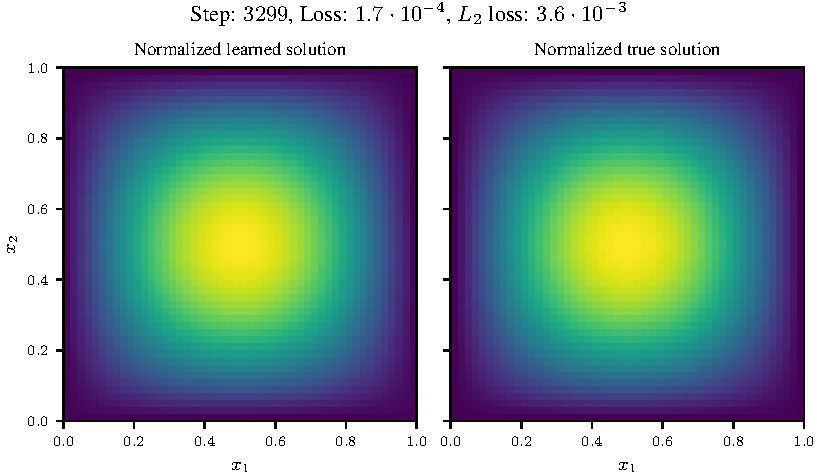
\includegraphics[width=\linewidth]{../kfac_pinns_exp/exp42_visualize_solutions/visualize_solution/SGD/poisson_2d_sin_product_mlp-tanh-64_SGD_step0003299.pdf}%
          \newframe[1.0]%
          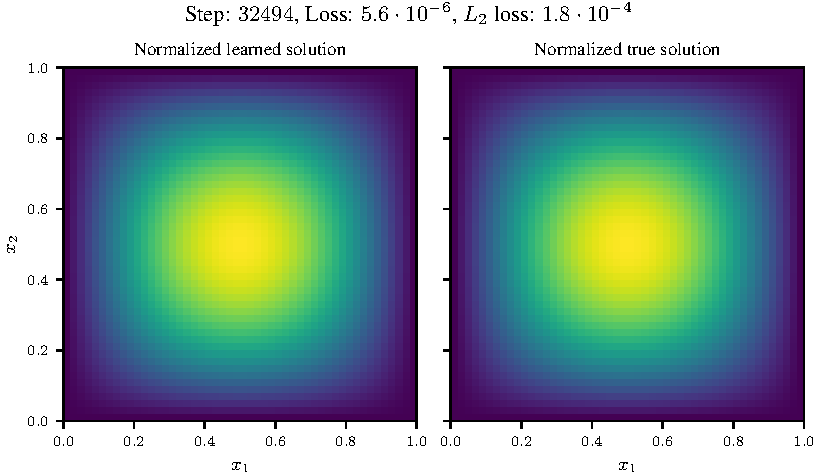
\includegraphics[width=\linewidth]{../kfac_pinns_exp/exp42_visualize_solutions/visualize_solution/SGD/poisson_2d_sin_product_mlp-tanh-64_SGD_step0032494.pdf}%
        \end{animateinline}
      }
      \only<4>{%
        \vspace{0.5ex}

        \emph{Hard to train with popular methods}

        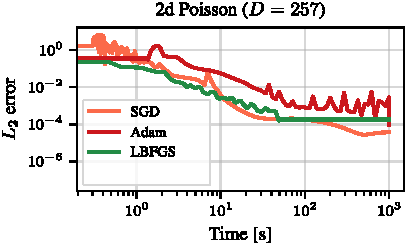
\includegraphics[width=0.9\linewidth]{figures/poisson2d-01.pdf}
        \vspace{1ex}
      }
      \only<5>{%
        \vspace{0.5ex}

        \emph{2\textsuperscript{nd}-order works} {\scriptsize \citep[][ICML]{muller2023achieving}}

        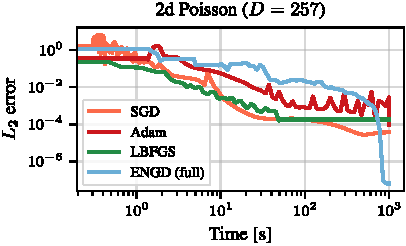
\includegraphics[width=0.9\linewidth]{figures/poisson2d-02.pdf}
        \vspace{1ex}
      }
      \only<6>{%
        \vspace{0.5ex}

        \emph{but proposed methods don't scale}

        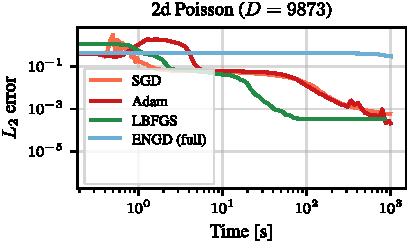
\includegraphics[width=0.9\linewidth]{figures/poisson2d-medium-01.pdf}
        \vspace{1ex}
      }
      \only<7>{%
        \vspace{0.5ex}

        \emph{We derive KFAC, which scales well}

        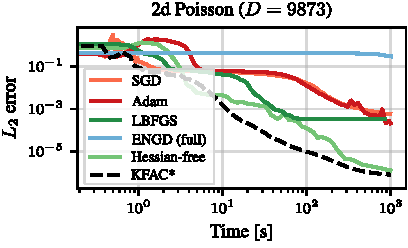
\includegraphics[width=0.9\linewidth]{figures/poisson2d-medium-03.pdf}
        \vspace{1ex}
      }
      \vspace*{-5.5ex}
    \end{column}
  \end{columns}

  \uncover<3->{
    \begin{align*}
      \min_{\vtheta}
      L(\vtheta)
      \coloneqq
      \underbrace{
      \frac{1}{2N_{\Omega}} \sum_{n=1}^{N_{\Omega}}
      \left(
      \hat{\gL}u_{\vtheta}(\vx_n) - f(\vx_n)
      \right)^2
      }_{L_{\Omega}(\vtheta)}
      +
      \underbrace{
      \frac{1}{2N_{\partial\Omega}} \sum_{n=1}^{N_{\partial\Omega}}
      \left(
      u_{\vtheta}(\vx_n^{\text{b}}) - g(\vx_n^{\text{b}})
      \right)^2
      }_{L_{\partial\Omega}(\vtheta)}
    \end{align*}
  }
\end{frame}
%%% Local Variables:
%%% mode: LaTeX
%%% TeX-master: "../main"
%%% End:
